%  LaTeX support: latex@mdpi.com 
%  For support, please attach all files needed for compiling as well as the log file, and specify your operating system, LaTeX version, and LaTeX editor.

%=================================================================
\documentclass[journal,article,submit,moreauthors,pdftex]{Definitions/mdpi} 

% For posting an early version of this manuscript as a preprint, you may use "preprints" as the journal and change "submit" to "accept". The document class line would be, e.g., \documentclass[preprints,article,accept,moreauthors,pdftex]{mdpi}. This is especially recommended for submission to arXiv, where line numbers should be removed before posting. For preprints.org, the editorial staff will make this change immediately prior to posting.

%--------------------
% Class Options:
%--------------------
%----------
% journal
%----------
% Choose between the following MDPI journals:
% acoustics, actuators, addictions, admsci, adolescents, aerospace, agriculture, agriengineering, agronomy, ai, algorithms, allergies, analytica, animals, antibiotics, antibodies, antioxidants, appliedchem, applmech, applmicrobiol, applnano, applsci, arts, asi, atmosphere, atoms, audiolres, automation, axioms, batteries, bdcc, behavsci, beverages, biochem, bioengineering, biologics, biology, biomechanics, biomedicines, biomedinformatics, biomimetics, biomolecules, biophysica, biosensors, biotech, birds, bloods, brainsci, buildings, businesses, cancers, carbon, cardiogenetics, catalysts, cells, ceramics, challenges, chemengineering, chemistry, chemosensors, chemproc, children, civileng, cleantechnol, climate, clinpract, clockssleep, cmd, coatings, colloids, compounds, computation, computers, condensedmatter, conservation, constrmater, cosmetics, crops, cryptography, crystals, curroncol, cyber, dairy, data, dentistry, dermato, dermatopathology, designs, diabetology, diagnostics, digital, disabilities, diseases, diversity, dna, drones, dynamics, earth, ebj, ecologies, econometrics, economies, education, ejihpe, electricity, electrochem, electronicmat, electronics, encyclopedia, endocrines, energies, eng, engproc, entropy, environments, environsciproc, epidemiologia, epigenomes, fermentation, fibers, fire, fishes, fluids, foods, forecasting, forensicsci, forests, fractalfract, fuels, futureinternet, futuretransp, futurepharmacol, futurephys, galaxies, games, gases, gastroent, gastrointestdisord, gels, genealogy, genes, geographies, geohazards, geomatics, geosciences, geotechnics, geriatrics, hazardousmatters, healthcare, hearts, hemato, heritage, highthroughput, histories, horticulturae, humanities, hydrogen, hydrology, hygiene, idr, ijerph, ijfs, ijgi, ijms, ijns, ijtm, ijtpp, immuno, informatics, information, infrastructures, inorganics, insects, instruments, inventions, iot, j, jcdd, jcm, jcp, jcs, jdb, jfb, jfmk, jimaging, jintelligence, jlpea, jmmp, jmp, jmse, jne, jnt, jof, joitmc, jor, journalmedia, jox, jpm, jrfm, jsan, jtaer, jzbg, kidney, land, languages, laws, life, liquids, literature, livers, logistics, lubricants, machines, macromol, magnetism, magnetochemistry, make, marinedrugs, materials, materproc, mathematics, mca, measurements, medicina, medicines, medsci, membranes, metabolites, metals, metrology, micro, microarrays, microbiolres, micromachines, microorganisms, minerals, mining, modelling, molbank, molecules, mps, mti, nanoenergyadv, nanomanufacturing, nanomaterials, ncrna, network, neuroglia, neurolint, neurosci, nitrogen, notspecified, nri, nursrep, nutrients, obesities, oceans, ohbm, onco, oncopathology, optics, oral, organics, osteology, oxygen, parasites, parasitologia, particles, pathogens, pathophysiology, pediatrrep, pharmaceuticals, pharmaceutics, pharmacy, philosophies, photochem, photonics, physchem, physics, physiolsci, plants, plasma, pollutants, polymers, polysaccharides, proceedings, processes, prosthesis, proteomes, psych, psychiatryint, publications, quantumrep, quaternary, qubs, radiation, reactions, recycling, regeneration, religions, remotesensing, reports, reprodmed, resources, risks, robotics, safety, sci, scipharm, sensors, separations, sexes, signals, sinusitis, smartcities, sna, societies, socsci, soilsystems, solids, sports, standards, stats, stresses, surfaces, surgeries, suschem, sustainability, symmetry, systems, taxonomy, technologies, telecom, textiles, thermo, tourismhosp, toxics, toxins, transplantology, traumas, tropicalmed, universe, urbansci, uro, vaccines, vehicles, vetsci, vibration, viruses, vision, water, wevj, women, world 

%---------
% article
%---------
% The default type of manuscript is "article", but can be replaced by: 
% abstract, addendum, article, book, bookreview, briefreport, casereport, comment, commentary, communication, conferenceproceedings, correction, conferencereport, entry, expressionofconcern, extendedabstract, datadescriptor, editorial, essay, erratum, hypothesis, interestingimage, obituary, opinion, projectreport, reply, retraction, review, perspective, protocol, shortnote, studyprotocol, systematicreview, supfile, technicalnote, viewpoint, guidelines, registeredreport, tutorial
% supfile = supplementary materials

%----------
% submit
%----------
% The class option "submit" will be changed to "accept" by the Editorial Office when the paper is accepted. This will only make changes to the frontpage (e.g., the logo of the journal will get visible), the headings, and the copyright information. Also, line numbering will be removed. Journal info and pagination for accepted papers will also be assigned by the Editorial Office.

%------------------
% moreauthors
%------------------
% If there is only one author the class option oneauthor should be used. Otherwise use the class option moreauthors.

%---------
% pdftex
%---------
% The option pdftex is for use with pdfLaTeX. If eps figures are used, remove the option pdftex and use LaTeX and dvi2pdf.

%=================================================================
% MDPI internal commands
\firstpage{1} 
\makeatletter 
\setcounter{page}{\@firstpage} 
\makeatother
\pubvolume{1}
\issuenum{1}
\articlenumber{0}
\pubyear{2021}
\copyrightyear{2021}
%\externaleditor{Academic Editor: Firstname Lastname} % For journal Automation, please change Academic Editor to "Communicated by"
\datereceived{} 
\dateaccepted{} 
\datepublished{} 
\hreflink{https://doi.org/} % If needed use \linebreak
%------------------------------------------------------------------
% The following line should be uncommented if the LaTeX file is uploaded to arXiv.org
%\pdfoutput=1

%=================================================================
% Add packages and commands here. The following packages are loaded in our class file: fontenc, inputenc, calc, indentfirst, fancyhdr, graphicx, epstopdf, lastpage, ifthen, lineno, float, amsmath, setspace, enumitem, mathpazo, booktabs, titlesec, etoolbox, tabto, xcolor, soul, multirow, microtype, tikz, totcount, changepage, paracol, attrib, upgreek, cleveref, amsthm, hyphenat, natbib, hyperref, footmisc, url, geometry, newfloat, caption

%=================================================================
%% Please use the following mathematics environments: Theorem, Lemma, Corollary, Proposition, Characterization, Property, Problem, Example, ExamplesandDefinitions, Hypothesis, Remark, Definition, Notation, Assumption
%% For proofs, please use the proof environment (the amsthm package is loaded by the MDPI class).

%=================================================================
% Full title of the paper (Capitalized)
\Title{A causal web between chronotype and metabolic health traits}

% MDPI internal command: Title for citation in the left column
\TitleCitation{Title}

% Author Orchid ID: enter ID or remove command
\newcommand{\orcidauthorF}{0000-0002-0906-1323}
\newcommand{\orcidauthorB}{0000-0002-9588-6304}
\newcommand{\orcidauthorC}{0000-0001-8878-8434}
\newcommand{\orcidauthorD}{0000-0002-2705-2068}
\newcommand{\orcidauthorE}{0000-0002-6169-0135}
\newcommand{\orcidauthorA}{0000-0002-0357-5454}
\newcommand{\orcidauthorG}{0000-0003-2735-7010}
\newcommand{\orcidauthorH}{0000-0002-2061-091X}

%\newcommand{\orcidauthorA}{0000-0000-0000-000X} % Add \orcidA{} behind the author's name
%\newcommand{\orcidauthorB}{0000-0000-0000-000X} % Add \orcidB{} behind the author's name

% Authors, for the paper (add full first names)
\Author{John A. Williams $^{1,2}$ \orcidA{}*,   Dominic Russ $^{1,2}$\orcidD{}, Laura Bravo-Merodio $^{1,2}$ \orcidC{}, Victor Roth Cardoso $^{1,2}$ \orcidB{}, Samantha C. Pendleton $^{1,2}$ \orcidE{}, Furqan Aziz $^{1,2}$ \orcidF{},  Animesh Acharjee $^{1,2,3,}$ \orcidG{}, and Georgios V. Gkoutos $^{1,2,3,4, 5,6}$ \orcidH{}}

\AuthorNames{John A. Williams,  Dominic Russ, Laura Bravo-Merodio, Victor Roth Cardoso, Samantha C. Pendleton, Furqan Aziz,  Animesh Acharjee, and Georgios V. Gkoutos}


% MDPI internal command: Authors, for metadata in PDF
%\AuthorNames{Firstname Lastname, Firstname Lastname and Firstname Lastname}

% MDPI internal command: Authors, for citation in the left column
\AuthorCitation{Lastname, F.; Lastname, F.; Lastname, F.}
% If this is a Chicago style journal: Lastname, Firstname, Firstname Lastname, and Firstname Lastname.

\address{%
$^{1}$ Institute of Cancer and Genomic Sciences, Centre for Computational Biology, University of Birmingham, B15 2TT, UK\\
$^{2}$ Institute of Translational Medicine, University of Birmingham, B15 2TT, UK\\
$^{3}$ NIHR Surgical Reconstruction and Microbiology Research Centre, University Hospital Birmingham, Birmingham B15 2WB, UK\\
$^{4}$ MRC Health Data Research UK (HDR UK)\\
$^{5}$ NIHR Experimental Cancer Medicine Centre, B15 2TT, Birmingham, UK\\
$^{6}$ NIHR Biomedical Research Centre, University Hospital Birmingham, Birmingham, B15 2WB, UK}

% Contact information of the corresponding author
\corres{Correspondence: j.a.williams@bham.ac.uk}

% Current address and/or shared authorship
%\firstnote{Current address: Affiliation 3} 
%\secondnote{These authors contributed equally to this work.}
% The commands \thirdnote{} till \eighthnote{} are available for further notes

%\simplesumm{} % Simple summary

%\conference{} % An extended version of a conference paper

% Abstract (Do not insert blank lines, i.e. \\) 
\abstract{A single paragraph of about 200 words maximum. For research articles, abstracts should give a pertinent overview of the work. We strongly encourage authors to use the following style of structured abstracts, but without headings: (1) Background: place the question addressed in a broad context and highlight the purpose of the study; (2) Methods: describe briefly the main methods or treatments applied; (3) Results: summarize the article's main findings; (4) Conclusion: indicate the main conclusions or interpretations. The abstract should be an objective representation of the article, it must not contain results which are not presented and substantiated in the main text and should not exaggerate the main conclusions.}

% Keywords
\keyword{Circadian rhythm; Chronotype; Diabetes; Alcohol intake; Mendelian randomization} 

% The fields PACS, MSC, and JEL may be left empty or commented out if not applicable
%\PACS{J0101}
%\MSC{}
%\JEL{}

%%%%%%%%%%%%%%%%%%%%%%%%%%%%%%%%%%%%%%%%%%
% Only for the journal Diversity
%\LSID{\url{http://}}

%%%%%%%%%%%%%%%%%%%%%%%%%%%%%%%%%%%%%%%%%%
% Only for the journal Applied Sciences:
%\featuredapplication{Authors are encouraged to provide a concise description of the specific application or a potential application of the work. This section is not mandatory.}
%%%%%%%%%%%%%%%%%%%%%%%%%%%%%%%%%%%%%%%%%%

%%%%%%%%%%%%%%%%%%%%%%%%%%%%%%%%%%%%%%%%%%
% Only for the journal Data:
%\dataset{DOI number or link to the deposited data set in cases where the data set is published or set to be published separately. If the data set is submitted and will be published as a supplement to this paper in the journal Data, this field will be filled by the editors of the journal. In this case, please make sure to submit the data set as a supplement when entering your manuscript into our manuscript editorial system.}

%\datasetlicense{license under which the data set is made available (CC0, CC-BY, CC-BY-SA, CC-BY-NC, etc.)}

%%%%%%%%%%%%%%%%%%%%%%%%%%%%%%%%%%%%%%%%%%
% Only for the journal Toxins
%\keycontribution{The breakthroughs or highlights of the manuscript. Authors can write one or two sentences to describe the most important part of the paper.}

%%%%%%%%%%%%%%%%%%%%%%%%%%%%%%%%%%%%%%%%%%
% Only for the journal Encyclopedia
%\encyclopediadef{Instead of the abstract}
%\entrylink{The Link to this entry published on the encyclopedia platform.}
%%%%%%%%%%%%%%%%%%%%%%%%%%%%%%%%%%%%%%%%%%

\begin{document}
%%%%%%%%%%%%%%%%%%%%%%%%%%%%%%%%%%%%%%%%%%
%\setcounter{section}{-1} %% Remove this when starting to work on the template.
% \section{How to Use this Template}

% The template details the sections that can be used in a manuscript. Note that the order and names of article sections may differ from the requirements of the journal (e.g., the positioning of the Materials and Methods section). Please check the instructions on the authors' page of the journal to verify the correct order and names. For any questions, please contact the editorial office of the journal or support@mdpi.com. For LaTeX-related questions please contact latex@mdpi.com.
% %The order of the section titles is: Introduction, Materials and Methods, Results, Discussion, Conclusions for these journals: aerospace,algorithms,antibodies,antioxidants,atmosphere,axioms,biomedicines,carbon,crystals,designs,diagnostics,environments,fermentation,fluids,forests,fractalfract,informatics,information,inventions,jfmk,jrfm,lubricants,neonatalscreening,neuroglia,particles,pharmaceutics,polymers,processes,technologies,viruses,vision

\section{Introduction}



%%%%%%%%%%%%%%%%%%%%%%%%%%%%%%%%%%%%%%%%%%
\section{Materials and Methods}
A general workflow for the several MR studies in this chapter are depicted in Figure \ref{fig:MR_Workflow}. Data can be acquired from previously performed GWAS studies with data deposited in the GWAS Catalog, MR Base, or another database. Additionally, researchers may conduct their own GWAS using data they have available. I have done this in order to ensure that I include appropriate covariates during the GWAS itself. Next, to ensure sample independence, the UKBB population is split into two groups randomly, each with half the population. Then GWAS are conducted and held for further analysis. A discovery set of SNPs are obtained from an outside data source. Next, effect sizes and their variance from each GWAS are extracted for the discovery SNP loci. Data are then combined, and the effect sizes meta-analyzed to produce an MR study. Lastly, post-hoc analyses are performed to test for pleiotropy, directionality of effect between exposure and outcome, and the influence of specific SNPs in the model.

\begin{figure}[htbp]
	\centering
	\includegraphics[width=0.5\linewidth]{chapter3/HighRes_Fig_Tables/Signif/MR_workflow.pdf}
	\caption[Mendelian randomization workflow]{Mendelian Randomization workflow for testing the causal influence of Evening Chronotype on psychosocial and vision traits from the UK Biobank (UKBB). Discovery SNPs associating with chronotype are obtained from an outside population. The UKBB is split into exposure, which has a GWAS performed against Chronotype, and Outcome, which has a GWAS performed against another trait. Discovery SNPs or proxies are extracted from each GWAS, using clumping to ensure SNP independence. Data are combined, and an IVW meta-analysis of effect sizes from GWAS is performed, followed by tests for pleiotropy, directionality, and sensitivity. SNPs = single nucleotide polymorphisms, LD = linkage disequilibrium, GWAS = genome wide association study, IVW = inverse-variance weighted.}
	\label{fig:MR_Workflow}
\end{figure}

\subsection{Data Acquisition}
To obtain an unbiased set of SNPs which associate to chronotype, I downloaded all significant (<= 9.000e-6) variants from a 2016 GWAS conducted by 23andMe \citep{hu_gwas_2016} via GWAS Catalog \citep{gwas_catalog}, accession GCST00342, a total of 77 SNPs on 20 Jan, 2020. 

\subsubsection{Experimental Data}
The UK Biobank (UKBB) \citep{bycroft_uk_2018} was initially proposed by the Wellcome Trust and the Medical Research Council, with the goal of identifying risk factors for human disease \citep{collins_what_2012}. The resource focuses on middle age adults, largely of European descent. A plethora of biological samples and exams were taken from each subject, including genetic material, magnetic resonance imaging (MRI) of several body regions, health and lifestyle questionnaires, and medical history data. The UKBB aims to recruit 500,000 individuals, a large sample size reflecting the likelihood of any one individual developing a given disorder or disease \citep{collins_what_2012}. Participants signed electronic concent declarations, and the UKBB received ethics approval \citep{bycroft_uk_2018}. For a full description of the resource and every measure available for use upon approved application, see https://biobank.ctsu.ox.ac.uk/crystal/, with further details available as reported previously \citep{bycroft_uk_2018,collins_what_2012}. The research in this chapter was performed under project number 31224. 

UK resident participants registered with the National Health Service (NHS) were recruited between 40 and 69 years of age between 2006 and 2010. At baseline, participants donated blood and urine, and completed self assessment questionnaires relating to lifestyle, medical and family history \citep{allen_uk_2014,collins 2007}. As of July 2020, 488,264 participants have been recruited and genotyped. Participants completed self-guided questionnaires on centre computers with the aid of in-built help systems when prompted. Genetic data were extracted from blood as previously described \citep{bycroft_uk_2018,collins 2007}. Deoxyribonucleic acid (DNA) was extracted at baseline, and initial genetic data from Affymetrix arrays were released in May 2015 and July 2017 \citep{bycroft_uk_2018}. The first release included 150,000 participants, with 50,000 genotype using the Applied Biosystems UK Biobank Lung Exome Variant Evaluation  (UK BiLEVE) Axiom Array, and all other participants genotyped via the Applied Biosystems UK biobank Axiom Array  \citep{bycroft_uk_2018}. Both arrays share 95\% of markers. Genetic SNP arrays can use imputation to increase coverage, which was performed as described \citep{bycroft_uk_2018}. Multiallelic SNPs or those with a minor allele frequency (MAF) of < 0.01 (1\%) were removed prior to imputation, The UK10K and Haplotype Reference Consortium (HRC) reference pannels were the basis for imputation, performed by the MRC-IEU unit \citep{huang 2015, howie 2011}. Individuals self identifying as 'White British' and having similar ancestry by clustering with others of the same ancestry in PCA were included, while those with a high degree of kinship to others in the biobank were excluded. The MRC-IEU also preformed quality control during imputation, excluding individuals with a sex mismatch between self reported and genetics, or any individuals with sex-chromosome aneuploidy. For a full description of imputation, see \citep{bycroft_uk_2018}, and for a full description of in-house MRC-IEU quality control see \citep{ruth_mitchell_mrc_2019}. 

Phenotypic data were obtained for the following fields for use in three studies in this chapter (Table \ref{tab:Studies_MRchapter}). Three studies were conducted. First, a study of the influence of chronotype on self-reported mental health related traits. Then, a study of the effect of chronotype on social support and lifestyle factors. Lastly, a study encompassing the influence of chronotype on measures of eye health, taken by the best keratometry index measurements in the UKBB. When a categorical response has multiple values, they are separated into binary $1/0$ outcomes for individual analysis. 

\input{chapter3/HighRes_Fig_Tables/Signif/Studies_MRchapter}

\subsection{Performing GWAS}
After harmonizing outcomes, PLINKv1.9 was used to perform GWAS against each trait studied, including chronotype \citep{chang_second-generation_2015}. During each GWAS, the following procedure was followed.

Quality control was carried out using PLINK R v3.5.0 \citep{r_core_team_r:_2013}. Variants which had a particularly high missing call rate (>0.1) were removed. Individuals with a missing rate of > 0.05 were also excluded. A 50kb window with a step size of 5 variants at a time and a 0.5 r2 threshold was used to remove variants in high LD. 

Variants with a MAF <0.01 were also excluded. For each analysis, covariates included gender and the first ten principle components. PLINK was used to calculate the principal components using default settings. Prior to any testing, final QC steps were taken per trait, removing variants based on a case control missing rate likelihood of < 0.001 when a trait was binary, missing rate 0.05 or a Hardy Weinberg Equilibrium p < 1E-8. 

Linear models were run on all continuous traits, and logistic regression models were used for all binary traits. To make the comparison of effect sizes between binary and continuous outcomes efficient, the $\beta$ values from the generalized linear model during logistic regression were retained using PLINK's "--beta" flag. $\beta$, standard error ($se$), and p-values from each GWAS were kept for the data harmonization process.

\subsection{Data Harmonization}
When mining each GWAS for the discovery SNPs from 23andMe, a harmonization process was performed using the R TwoSampleMR package \citep{hemani_mr-base_2018}. First, SNPs from the discovery set were located in the exposure GWAS summary statistics. The strandedness of each GWAS was checked to make sure that at each allele, the minor and major alleles were equal. If these were reversed, effect sizes were modified to correct for this. Pallendromic SNPs, which contain alleles represented by the same base pairs on both strands of DNA, were discarded. If SNPs were not present, proxies were found using PLINK with an $R^2$ of at least 0.8, and strand was checked again \citep{plink}. Next, SNPs in the exposure GWAS set were clumped by LD to ensure statistical independence. In a window of 10000 base pairs, an $R^2$ cutoff of < 0.001 was set to obtain haplotype blocks, and the European reference panel of the 10,000 Genomes Project \citep{10kgenomes}. This left 18 SNPs for use as valid, independent IVs. The effect sizes and standard errors from each GWAS were extracted for these 18 SNPs used in this analysis. 

\subsection{Causal Inference Modelling}
In practice, meta-analyses often use an inverse-variance weighted average to account for the sample size (reflected in variance) of studies included in the meta-analysis. The IVW methods uses the Wald ratios of each SNPs as the "study" the meta-analysis, with a pooled estimate seen in the forest plots below (see results) driving home the meta-analytic nature of multi-SNP MR. Rather than calculate Wald ratios individually, the outcome GWAS $\beta$s or Odds Ratios are regressed on the exposure. The slope of the regression line indicates the strength of the effect, as an increase in the unit of outcome per unit of the exposure\cite{burgess_interpreting_2017}. 
In a IVW metaanalysis, IVW estimate is calculated by:
\begin{equaton}
\widehat{\beta}_{Yj} = \theta_{IVW}\widehat{\beta}_{Xj} + \epsilon_{Ij}; \epsilon_{Ij} \sim N(0,\sigma^2se(\widehat{\beta}_{Yj})^2)
\end{equaton}

where $\widehat{\theta}$ is the inverse variance weighted average, $se$ is the standard error, and other terms are as above, and I is an error term.



Similarly to other meta-analysis frameworks, by weighting effect sizes by their inverse variance, stronger SNPs make a larger contribution to the overall effect size obtained. Compared to other methods used in this analysis, the IVW method has the strongest power simply by not discarding any SNP instruments (Mode) or shrinking their variance (MR Egger). It strongly assumes all instruments are valid, requiring the slope of the meta-regression line to be constrained to zero. Any potential pleiotropy or extreme heterogeneity among SNPs would draw the gradient of the regression line away from the true slope. Heterogeneity can occur when individual SNPs do not converge on an estimate, and can be estimate by Cochran's $Q$ \citep{higgins_cochrane_2011}. In this context, heterogeneity may be a sign of horizontal pleiotropy, wherein SNPs effect the outcome by their influence on other confounding traits \cite{burgess_review_2017}. In any IVW-based meta-analysis, either fixed or random effects maybe modeled \cite{higgins_cochrane_2011}. A fixed effect model applied to MR assumes all instruments are valid, whereas modeling random effects allows for balanced horizontal pleiotropy to be present if it is independent of SNPs effects on the exposure. This is termed the Instrument Strength Independent of Direct Effect (InSIDE) assumption, which is not currently testable. The IVW method also relies on the No Measurement Error (NOME) assumption, assuming SNP-exposure associations are accurate. This can be accessed by calculating F-statistics to test the degree of association between discovery SNPs and the exposure of interest. 

A figure comparing the IVW method with the pleiotropy- and assumption-mitigating factors below is shown in \ref{fig:MR_Scatters}.  Each scatter plot depicts an outcome regressed on an exposure with multiple SNPs. The slope is the estimate of the causal effect. If there is no horizontal pleiotorpy, or the pleiotropy is balanced between outcome and effect, inverse-variance weighted regression is used, where the contribution of each SNP is weighted by its inverse variance, so variable SNPs contribute less to the overall study effect size. If directional pleiotropy is suspected, then constraining the intercept to be at zero will allow bias into the model (gray arrow). However if the intercept is not constrained via Egger regression, an unbiased estimate can be obtained if the instrument-exposure and pleiotropy are uncorrelated (InSIDE assumption). If most instruments are valid (black), and some are invalid (red), a median-based approach will provide an unbiased estimate (black), whereas IVW linear regression would provide a biased estimate (grey). If SNPs are horizontally pleiotropic, they will return biased estimates. Using a mode-based estimator, it is possible to clustering SNPs based on their estimates (grey lines). If the majority of the SNPs are in a cluster which satisfies IV assumptions, then then mode-based estimator is unbiased, if not under powered.

\begin{figure}[htbp]
	\centering
	\includegraphics[width=0.5\linewidth]{chapter3/HighRes_Fig_Tables/Signif/mod_elife-34408-fig1-v1.jpg}
	\caption[Mendelian Randomization Method Scatter Plots]{Mendelian Randomization methods have different assumptions. Each scatter plot depicts an outcome regressed on an exposure with multiple SNPs. The slope is the estimate of the causal effect. A) If there is no horizontal pleiotorpy, or the pleiotropy is balanced between outcome and effect, inverse-variance weighted regression is used, where the contribution of each SNP is weighted by its inverse variance, so variable SNPs contribute less to the overall study effect size. B) If directional pleiotropy is suspected, then constraining the intercept to be at zero will allow bias into the model (gray arrow). However if the intercept is not constrained via Egger regression, an unbiased estimate can be obtained if the instrument-exposure and pleiotropy are uncorrelated (InSIDE assumption). C) If most instruments are valid (black), and some are invalid (red), a median-based approach will provide an unbiased estimate (black), whereas IVW linear regression would provide a biased estimate (grey). D) If SNPs are horizontally pleiotropic, they will return biased estimates. Using a mode-based estimator, it is possible to clustering SNPs based on their estimates (grey lines). If the majority of the SNPs are in a cluster which satisfies IV assumptions, then then mode-based estimator is unbiased, if not under powered. Image credit: \cite{hemani_evaluating_2018}.}
	\label{fig:MR_Scatters}
\end{figure}

\subsection{Testing for Evidence of Pleiotropy}
When an MR study, with multiple valid instruments, is considered as a meta-analysis, meta-analytic tools used to detect bias in studies can be used to detect bias in SNPs. Egger proposed a method for detecting small study bias in meta-analyses, and this has been adopted into an MR context \citep{bowden_framework_2017,bowdenMendelianRandomizationInvalid2015b}. The Wald ratios of each SNP are used in meta-regression by taking the inverse IVW weights used in IVW analysis, without modeling the intercept. It provides a causal estimate similar to IVW but adjusted for horizontal pleiotropy which would otherwise invalidate IVW \cite{bowdenMendelianRandomizationInvalid2015b}. As the intercept is unconstrained, it estimates the average pleiotropic effect across the SNPs, and the slope provides an estimate of the pleiotropic effect. If the intercept, while not constrained, is not statistically different than zero, then this suggest lack of horizontal pleiotropy and the instruments are assumed valid. To accomplish this, the MR-Egger method relaxes assumption 3 in \ref{fig:MR_Dag}. MR-Egger relies on not violating the InSIDE assumption (see above). 

MR-Egger regression is an extension of IVW regression. Instead of assuming no intercept term, an intercept is estimated:
\begin{equation}
\widehat{\beta}_{Yj} = \theta_{0E} + \theta_{1E}\widehat{\beta}_{Xj} + \epsilon_{Ej}; \epsilon_{Ej} \sim N(0,\sigma^2se(\widehat{\beta}_{Yj})^2)
\end{equation}
where $\theta_{0E}$ is the intercept and $\theta_{1E}$ the MR Egger estimate.
If the intercept is equal to zero, then the IVW method and MR-Egger will be equivalent \citep{burgess_interpreting_2017}. During the IVW process in MR-Egger, the effect sizes of each SNP must have the same sign, and this decreases the variation between them \citep{bowdenMendelianRandomizationInvalid2015b}. This renders the MR-Egger method the lowest powered method employed in this chapter, though its robustness to horizontal pleiotropy and ability to test for this in the intercept make it a valuable contribution to methods. 


\subsection{Assuming Weak Instrumental Variables: Median and Mode}
The weighted median estimate again relies on Wald ratios. First, the Wald ratio is calculated for each SNP. Then, as in the IVW method, a measure of central tendancy is used to produce an overall effect size - but instead of the mean, the median is used. In an unweighted analysis it would be assumed that over half of the instruments are valid, while in an weighted median analysis the assumption is that the at least 50\% of the weight of the instruments are valid themselves \citep{bowden_consistent_2016}. This approach is robust to directional pleiotropy when compared to a simple IVW meta-analysis. It is also more robust to outliers than either IVW or Mr Egger. 

Comparative studies have demonstrated that the power of the weighted median method is similar to the IVW. Moreover, it is not constrained by the InSIDE assumption, contrary to MR Egger, and for it to be valid only half of instruments need to be unbiased \cite{hemani_evaluating_2018}.  See \ref{fig:MR_Scatters} C for a graphical explanation. 

The mode-based estimator (MBE) clusters Wald ratios before calculating random effects in an IVW meta-analysis \citep{hartwigRobustInferenceSummary2017a}. The simple MBE uses unweighted analysis, while the weighted MBE uses inverse variance weighting. First, a smooth empirical density function is calculated for each Wald ratio and are then clustered. The ZEMPA assumption (Zero Modal Pleiotropy Assumption) states that the biggest cluster with the same ratio estimates will be valid instruments. Thus, the MBE can provide a valid causal estimate when the largest number of estimates come from valid IVs, even if a majority (those in smaller clusters) are invalid. While not all snps have to be valid IVs, fewer valid IVs is equivalent to fewer samples actually used, and results in lost power compared to IVW methods. 
I calculated both weighted (by IVW) and unweighted (Wald ratio) methods. See \ref{fig:MR_Scatters} D for a graphical explanation. 

\subsection{Sensitivity, Bias, and Directionality}

To check if possible pleiotrophic or invalid SNPs are dominating models run, I performed a leave-one-out analysis for each experiment. In a leave-one-out senario, the inverse variance weighted average is run using all SNPs except one. This is repeated for every SNP, resulting in 10 IVW average effect sizes in the case of 10 SNPs in the analysis. One outlier effect size would indicate that the SNP left out skews the analysis and may be removed for being an outlier \citep{hemaniOrientingCausalRelationship2017}.

I composed funnel plots to access pleiotopic effects. Originally designed to identify potential biases arising from small studies in meta-analysis, funnel plots are a graphical method of accessing bias, by plotting the effect size against sample size, noting that smaller effects should belong to smaller effect sizes and that there should be a degree of balance in the signs of the effect sizes \citep{eggerBiasMetaanalysisDetected1997a}. Egger proposed a regression method to test the asymmetry of this relationship, which is the basis of the MR Egger method \citep{bowdenMendelianRandomizationInvalid2015b}. Cochran's $Q$ can be used in combination with funnel plots to access the degree of pleiotropy. $Q$ is a measure of heterogeneity among calculates the sum of squared differences between SNPs and the pooled effect, and creates a $\chi^2$ test statistic for comparison. The $Q$ statistic is well powered as the number of SNPs increases, indicating that evidence of overdispersion itself does not indicate pleiotropy \citep{Lawlor_2008,Rees_wood, burgess_review_2017}. Even for a low p-value, indicating high heterogeneity, I have investigated funnel plots, as severe asymmetry would suggest directional pleiotropy and violate MR-IVW assumptions. If symmetry is observed, both fixed- and random-effects IVW would produce similar results \cite{bowden_framework_2017}, and if asymmetry is observed then estimates would differ, and Median or Mode methods should be considered. In this chapter, the IVW analysis is considred the gold standard; if it is significant, other methods are used to confirm results in the presence of pleiotropy or heterogeneity. If all methods of analysis for an experiment concur, the potential causal effect of chronotype is considered more plausible.

I used the Steiger test to access the directional of all causative analyses post-hoc \citep{hemaniOrientingCausalRelationship2017}.  This method tests whether the selected IVs are more strongly associated with the exposure than the outcome. The Steiger test first assesses which variables (exposure or outcome) are influenced by the SNPs used, by testing if the SNPs explain more variance in the exposure than in the outcome with a modified $Z$ statistic. If the p-value of the IVW estimate and the Steiger estimate are both significant, the sign of the $Z$ statistic is used to assign the correct causal direction between exposure and outcome.




%%%%%%%%%%%%%%%%%%%%%%%%%%%%%%%%%%%%%%%%%%
\section{Results}

All figures and tables should be cited in the main text as Figure~\ref{forestIVW}, Table~\ref{tab1}, etc.

\subsection{To remove: database-minded chronotype - trait relationships}

%% table: traits with genome-wide signifiance in EpiGraphDB

%% figure: re-analysis forest plots of significant traits

\begin{figure}[htbp]
	\centering
	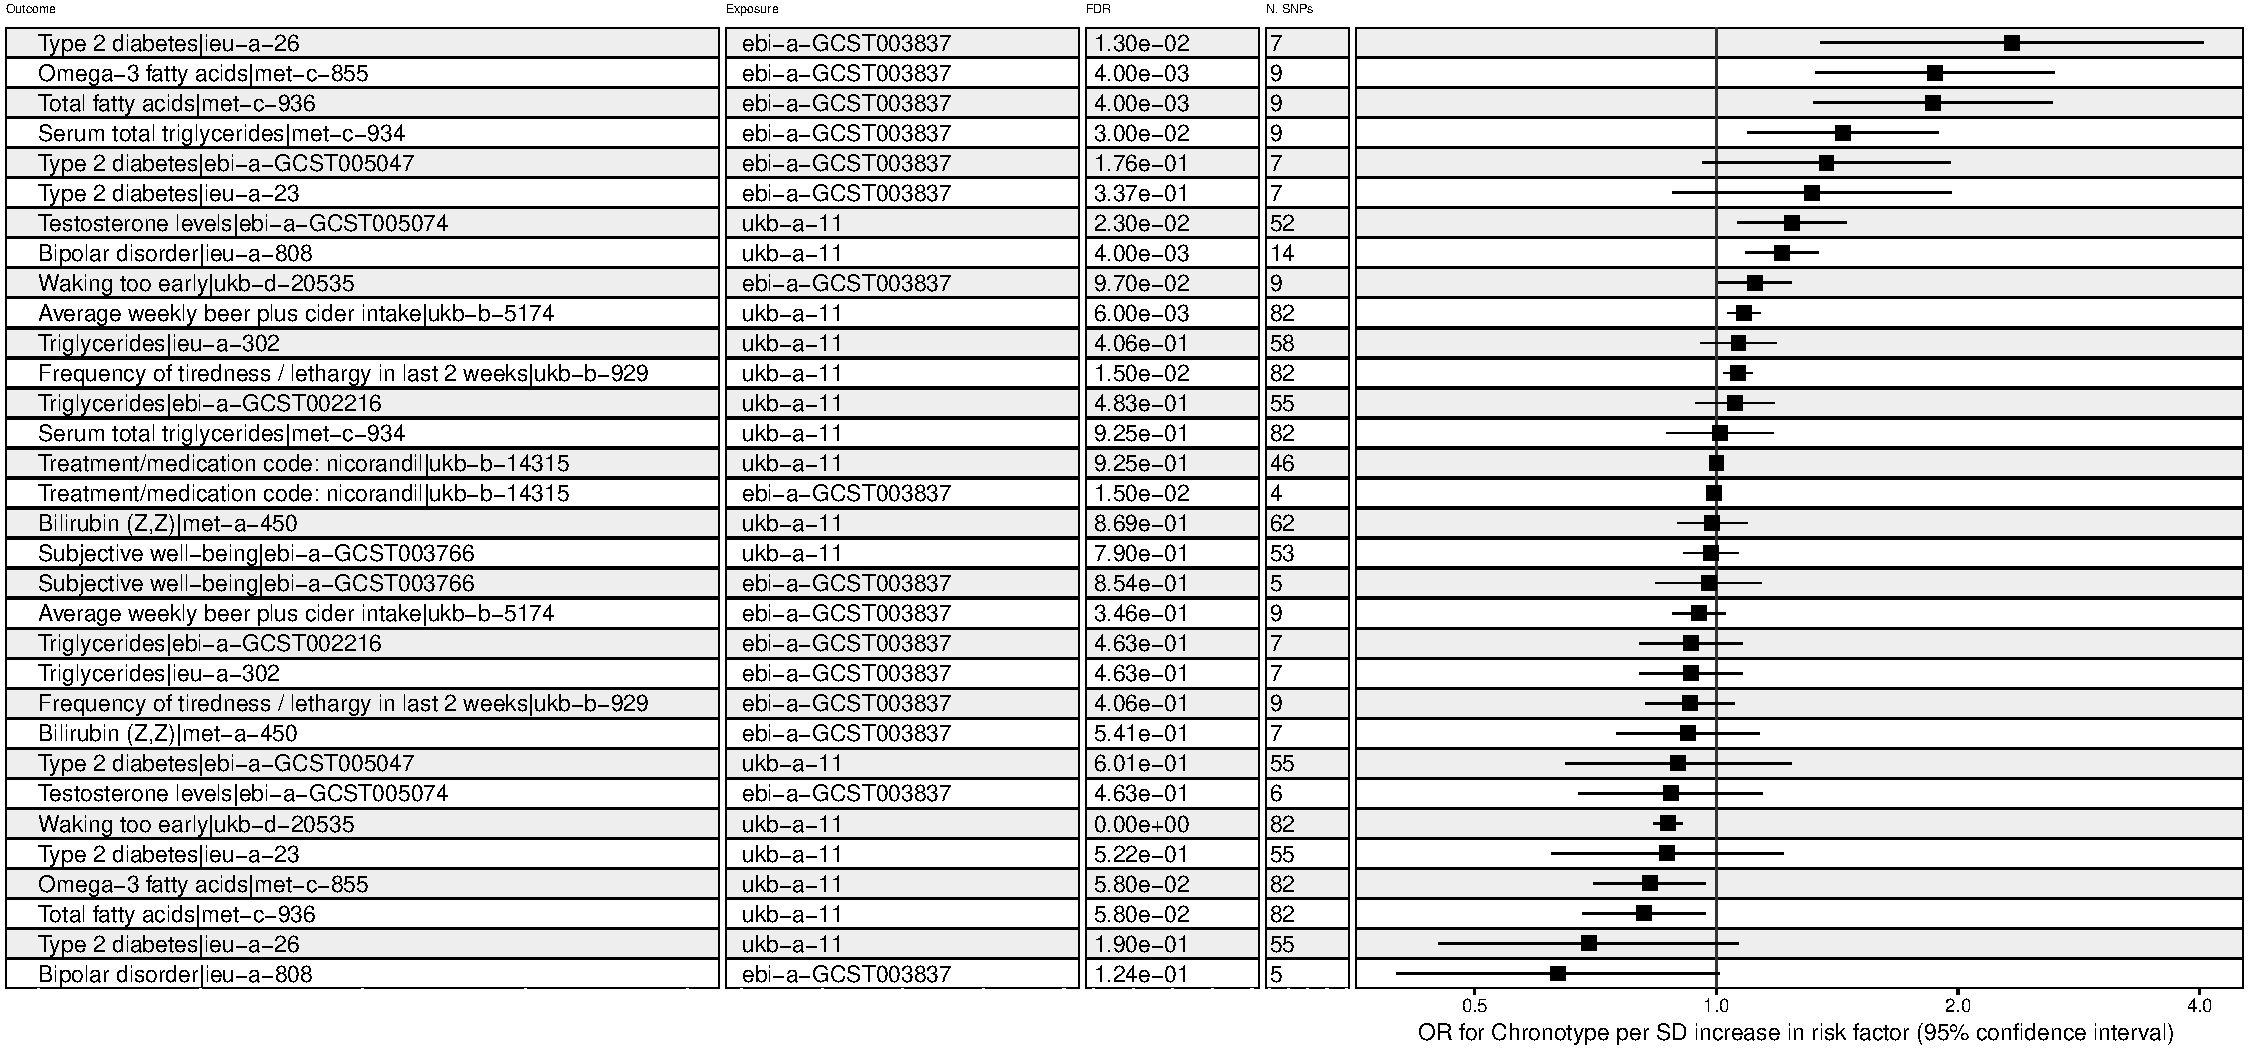
\includegraphics[width=0.5\linewidth]{Figs/forestIVW.pdf}
	\caption{Causal relationshps between exposure to chronotype and various traits. Causal associations mined from EpiGraphDB (IVW p < 5e-8) were analyzed using two chronotype exposure measures. Outcomes are listed with trait and study accession number. Exposure ebi-a-GCST003837 reflects SD increase in chronotype on a continuous morning - evening scale. Exosure ukb-a-11 represents odds of an evening chronotype. Effect sizes are from fixed-effects inverse variance weighted analyses with 95\% confidence intervals. False discovery rate-corrected pvalues are shown.}
	\label{forestIVW}
\end{figure}

\subsection{}







%%%%%%%%%%%%%%%%%%%%%%%%%%%%%%%%%%%%%%%%%%
\section{Discussion}



%%%%%%%%%%%%%%%%%%%%%%%%%%%%%%%%%%%%%%%%%%
\section{Conclusions}



%%%%%%%%%%%%%%%%%%%%%%%%%%%%%%%%%%%%%%%%%%
% \section{Patents}

% This section is not mandatory, but may be added if there are patents resulting from the work reported in this manuscript.

%%%%%%%%%%%%%%%%%%%%%%%%%%%%%%%%%%%%%%%%%%
\vspace{6pt} 

%%%%%%%%%%%%%%%%%%%%%%%%%%%%%%%%%%%%%%%%%%
%% optional
%\supplementary{The following are available online at \linksupplementary{s1}, Figure S1: title, Table S1: title, Video S1: title.}

% Only for the journal Methods and Protocols:
% If you wish to submit a video article, please do so with any other supplementary material.
% \supplementary{The following are available at \linksupplementary{s1}, Figure S1: title, Table S1: title, Video S1: title. A supporting video article is available at doi: link.} 

%%%%%%%%%%%%%%%%%%%%%%%%%%%%%%%%%%%%%%%%%%
\authorcontributions{\authorcontributions{Conceptualization, J.A.W.; methodology, J.A.W.; software, J.A.W; validation J.A.W.; formal analysis J.A.W.; investigation, J.A.W., D.R., V.R.C., L.B.M., S.P., F.A., A.A., G.V.G.; writing–original draft preparation, J.A.W, G.V.G; writing–review and editing,J.A.W., D.R., V.R.C., L.B.M., S.P., F.A., A.A., G.V.G.; visualization, J.A.W.; supervision, A.A., G.V.G; project administration, G.V.G; funding acquisition, G.V.G.}}
%For research articles with several authors, a short paragraph specifying their individual contributions must be provided. The following statements should be used ``Conceptualization, X.X. and Y.Y.; methodology, X.X.; software, X.X.; validation, X.X., Y.Y. and Z.Z.; formal analysis, X.X.; investigation, X.X.; resources, X.X.; data curation, X.X.; writing---original draft preparation, X.X.; writing---review and editing, X.X.; visualization, X.X.; supervision, X.X.; project administration, X.X.; funding acquisition, Y.Y. All authors have read and agreed to the published version of the manuscript.'', please turn to the  \href{http://img.mdpi.org/data/contributor-role-instruction.pdf}{CRediT taxonomy} for the term explanation. Authorship must be limited to those who have contributed substantially to the work~reported.}

\funding{The authors acknowledge support from the NIHR Birmingham ECMC, NIHR Birmingham SRMRC, Nanocommons H2020-EU (731032) and the NIHR Birmingham Biomedical Research Centre and the MRC Heath Data Research UK (HDRUK/CFC/01), an initiative funded by UK Research and Innovation, Department of Health and Social Care (England) and the devolved administrations, and leading medical research charities. The views expressed in this publication are those of the authors and not necessarily those of the NHS, the National Institute for Health Research, the Medical Research Council or the Department of Health.}

%\institutionalreview{In this section, please add the Institutional Review Board Statement and approval number for studies involving humans or animals. Please note that the Editorial Office might ask you for further information. Please add ``The study was conducted according to the guidelines of the Declaration of Helsinki, and approved by the Institutional Review Board (or Ethics Committee) of NAME OF INSTITUTE (protocol code XXX and date of approval).'' OR ``Ethical review and approval were waived for this study, due to REASON (please provide a detailed justification).'' OR ``Not applicable'' for studies not involving humans or animals. You might also choose to exclude this statement if the study did not involve humans or animals.}

%\informedconsent{Any research article describing a study involving humans should contain this statement. Please add ``Informed consent was obtained from all subjects involved in the study.'' OR ``Patient consent was waived due to REASON (please provide a detailed justification).'' OR ``Not applicable'' for studies not involving humans. You might also choose to exclude this statement if the study did not involve humans.

%Written informed consent for publication must be obtained from participating patients who can be identified (including by the patients themselves). Please state ``Written informed consent has been obtained from the patient(s) to publish this paper'' if applicable.}

\dataavailability{Data are available via the EpiGraphDB and MRBase APIs.} 

%\acknowledgments{In this section you can acknowledge any support given which is not covered by the author contribution or funding sections. This may include administrative and technical support, or donations in kind (e.g., materials used for experiments).}

\conflictsofinterest{The authors declare no conflict of interest.} 

%% Optional
%\sampleavailability{Samples of the compounds ... are available from the authors.}

%%%%%%%%%%%%%%%%%%%%%%%%%%%%%%%%%%%%%%%%%%
%% Only for journal Encyclopedia
%\entrylink{The Link to this entry published on the encyclopedia platform.}

%%%%%%%%%%%%%%%%%%%%%%%%%%%%%%%%%%%%%%%%%%
%% Optional
\abbreviations{The following abbreviations are used in this manuscript:\\

\noindent 
\begin{tabular}{@{}ll}
MDPI & Multidisciplinary Digital Publishing Institute\\
DOAJ & Directory of open access journals\\
TLA & Three letter acronym\\
LD & Linear dichroism
\end{tabular}}

%%%%%%%%%%%%%%%%%%%%%%%%%%%%%%%%%%%%%%%%%%
%% Optional
% \appendixtitles{no} % Leave argument "no" if all appendix headings stay EMPTY (then no dot is printed after "Appendix A"). If the appendix sections contain a heading then change the argument to "yes".
% \appendixstart
% \appendix
% \section{}
% \subsection{}
% The appendix is an optional section that can contain details and data supplemental to the main text---for example, explanations of experimental details that would disrupt the flow of the main text but nonetheless remain crucial to understanding and reproducing the research shown; figures of replicates for experiments of which representative data are shown in the main text can be added here if brief, or as Supplementary Data. Mathematical proofs of results not central to the paper can be added as an appendix.

% \begin{specialtable}[H] 
% %\tablesize{\scriptsize}
% \caption{This is a table caption. Tables should be placed in the main text near to the first time they are~cited.\label{tab1}}
% %\tablesize{} % You can specify the fontsize here, e.g., \tablesize{\footnotesize}. If commented out \small will be used.
% \begin{tabular}{ccc}
% \toprule
% \textbf{Title 1}	& \textbf{Title 2}	& \textbf{Title 3}\\
% \midrule
% Entry 1		& Data			& Data\\
% Entry 2		& Data			& Data\\
% \bottomrule
% \end{tabular}
% \end{specialtable}

% \section{}
% All appendix sections must be cited in the main text. In the appendices, Figures, Tables, etc. should be labeled, starting with ``A''---e.g., Figure A1, Figure A2, etc. 

%%%%%%%%%%%%%%%%%%%%%%%%%%%%%%%%%%%%%%%%%%
%\end{paracol}
\reftitle{References}

% Please provide either the correct journal abbreviation (e.g. according to the “List of Title Word Abbreviations” http://www.issn.org/services/online-services/access-to-the-ltwa/) or the full name of the journal.
% Citations and References in Supplementary files are permitted provided that they also appear in the reference list here. 

%=====================================
% References, variant A: external bibliography
%=====================================
\externalbibliography{yes}
\bibliography{references}

%=====================================
% References, variant B: internal bibliography
%=====================================
% \begin{thebibliography}{999}
% % Reference 1
% \bibitem[Author1(year)]{ref-journal}
% Author~1, T. The title of the cited article. {\em Journal Abbreviation} {\bf 2008}, {\em 10}, 142--149.
% % Reference 2
% \bibitem[Author2(year)]{ref-book1}
% Author~2, L. The title of the cited contribution. In {\em The Book Title}; Editor1, F., Editor2, A., Eds.; Publishing House: City, Country, 2007; pp. 32--58.
% % Reference 3
% \bibitem[Author3(year)]{ref-book2}
% Author 1, A.; Author 2, B. \textit{Book Title}, 3rd ed.; Publisher: Publisher Location, Country, 2008; pp. 154--196.
% % Reference 4
% \bibitem[Author4(year)]{ref-unpublish}
% Author 1, A.B.; Author 2, C. Title of Unpublished Work. \textit{Abbreviated Journal Name} stage of publication (under review; accepted; in~press).
% % Reference 5
% \bibitem[Author5(year)]{ref-communication}
% Author 1, A.B. (University, City, State, Country); Author 2, C. (Institute, City, State, Country). Personal communication, 2012.
% % Reference 6
% \bibitem[Author6(year)]{ref-proceeding}
% Author 1, A.B.; Author 2, C.D.; Author 3, E.F. Title of Presentation. In Title of the Collected Work (if available), Proceedings of the Name of the Conference, Location of Conference, Country, Date of Conference; Editor 1, Editor 2, Eds. (if available); Publisher: City, Country, Year (if available); Abstract Number (optional), Pagination (optional).
% % Reference 7
% \bibitem[Author7(year)]{ref-thesis}
% Author 1, A.B. Title of Thesis. Level of Thesis, Degree-Granting University, Location of University, Date of Completion.
% % Reference 8
% \bibitem[Author8(year)]{ref-url}
% Title of Site. Available online: URL (accessed on Day Month Year).
% \end{thebibliography}

% If authors have biography, please use the format below
%\section*{Short Biography of Authors}
%\bio
%{\raisebox{-0.35cm}{\includegraphics[width=3.5cm,height=5.3cm,clip,keepaspectratio]{Definitions/author1.pdf}}}
%{\textbf{Firstname Lastname} Biography of first author}
%
%\bio
%{\raisebox{-0.35cm}{\includegraphics[width=3.5cm,height=5.3cm,clip,keepaspectratio]{Definitions/author2.jpg}}}
%{\textbf{Firstname Lastname} Biography of second author}

% The following MDPI journals use author-date citation: Arts, Econometrics, Economies, Genealogy, Humanities, IJFS, JRFM, Laws, Religions, Risks, Social Sciences. For those journals, please follow the formatting guidelines on http://www.mdpi.com/authors/references
% To cite two works by the same author: \citeauthor{ref-journal-1a} (\citeyear{ref-journal-1a}, \citeyear{ref-journal-1b}). This produces: Whittaker (1967, 1975)
% To cite two works by the same author with specific pages: \citeauthor{ref-journal-3a} (\citeyear{ref-journal-3a}, p. 328; \citeyear{ref-journal-3b}, p.475). This produces: Wong (1999, p. 328; 2000, p. 475)

%%%%%%%%%%%%%%%%%%%%%%%%%%%%%%%%%%%%%%%%%%
%% for journal Sci
%\reviewreports{\\
%Reviewer 1 comments and authors’ response\\
%Reviewer 2 comments and authors’ response\\
%Reviewer 3 comments and authors’ response
%}
%%%%%%%%%%%%%%%%%%%%%%%%%%%%%%%%%%%%%%%%%%
\end{document}

